\documentclass[a4paper,11.5pt,table]{article}
\usepackage[textwidth=170mm, textheight=230mm, inner=20mm, top=20mm, bottom=30mm]{geometry}
\usepackage[normalem]{ulem}
\usepackage[utf8]{inputenc}
\usepackage[T1]{fontenc}
\PassOptionsToPackage{defaults=hu-min}{magyar.ldf}
\usepackage[magyar]{babel}
\usepackage{amsmath, amsthm,amssymb, paralist, tikz, multirow}
\usetikzlibrary{shapes.geometric, arrows, positioning, math, calc}
\begin{document}
	\begin{figure}[!h]
		\centering
		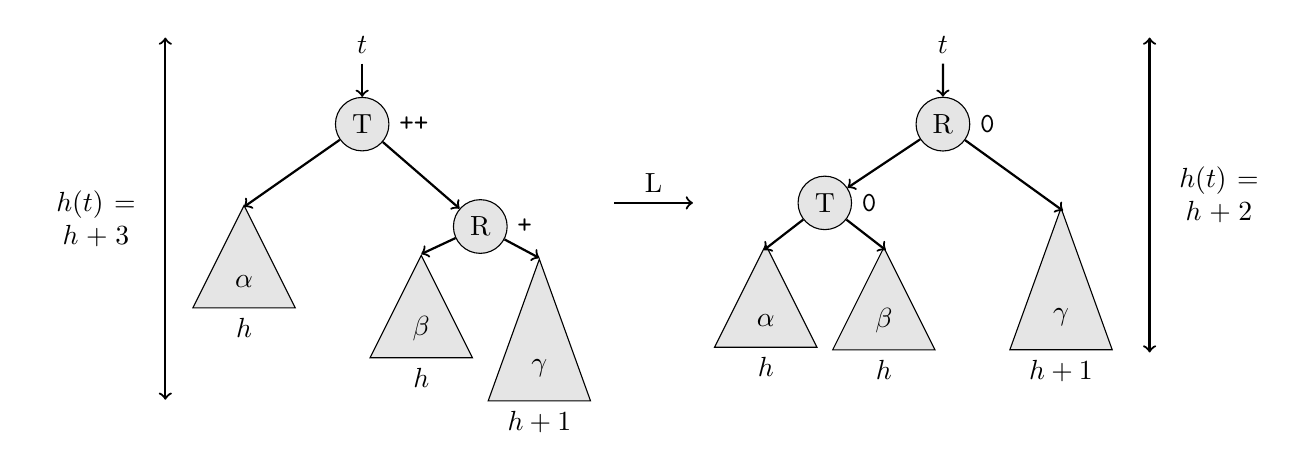
\begin{tikzpicture}[
				triangle/.style = {
					shape=isosceles triangle,
					shape border rotate = 90
				},
				level 1/.style={level distance=1cm},
				level 2/.style={sibling distance=3cm},
				level 3/.style={sibling distance=1.5cm},
				edge from parent/.style={draw=none}
			]
			\tikzstyle{Node} = [ %describes the basic look of the shapes
				text centered, 
				draw=black, 
				fill= gray!20
			]
			\tikzstyle{CircNode} = [
				circle,
				minimum width=6mm,
				Node
			]
			\tikzstyle{TriNode} = [
				triangle,
				minimum width=13mm, 
				minimum height=13mm,
				isosceles triangle stretches,
				Node
			]
			
			\node (t1) {$t$}
			child {
				node (T1) [CircNode]{T}
				child [level distance=20mm]{
					node (a1) [TriNode]{$\alpha$}
				}
				child [level distance=13mm]{
					node (R1) [CircNode]{R}
					child {
						node (b1) [TriNode]{$\beta$}
					}
					child [level distance = 18mm] {
						node (c1) [TriNode, minimum height=18mm]{$\gamma$}
					}
				}
			};
			\draw[->, thick] (t1) -- (T1);
			\draw[->, thick] (T1) -- (R1);
			\draw[->, thick] (T1) -- (-1.5,-2.05);
			\draw[->, thick] (R1) -- (0.75,-2.65);
			\draw[->, thick] (R1) -- (2.25,-2.7);
			\node [right = 0mm of T1] {\texttt{++}};
			\node [right = 0mm of R1] {\texttt{+}};
			\node [below = 0mm of a1] {$h$};
			\node [below = 0mm of b1] {$h$};
			\node [below = 0mm of c1] {$h+1$};
			\draw[<->, thick] (-2.5, -4.5) -- node [anchor=center, left, text width= 1.5cm, text centered]{$h(t)=$\\$h+3$}(-2.5, 0.1);
			
			\draw[->, thick] (3.2,-2) -- (4.2,-2) node [midway, above] {L};
			
			\node (t2)[right = 7 cm of t1] {$t$}
			child {
				node (R2) [CircNode]{R}
				child{
					node (T2) [CircNode] {T}
					[level distance = 15mm]
					child {
						node (a2) [TriNode]{$\alpha$}
					}
					child{
						node (b2)[TriNode]{$\beta$}
					}
				}
				child[level distance = 24.5mm] {
					node (c2) [TriNode, minimum height=18mm] {$\gamma$}
				}
			};
			\draw[->, thick] (t2) -- (R2);
			\draw[->, thick] (R2) -- (T2);
			\draw[->, thick] (T2) -- (5.1,-2.6);
			\draw[->, thick] (T2) -- (6.65,-2.6);
			\draw[->, thick] (R2) -- (8.9,-2.1);
			\node [right = 0mm of T2] {\texttt{0}};
			\node [right = 0mm of R2] {\texttt{0}};
			\node [below = 0mm of a2] {$h$};
			\node [below = 0mm of b2] {$h$};
			\node [below = 0mm of c2] {$h+1$};
			\draw[<->, thick] (10, -3.9) -- node [anchor=center, right, text width= 1.5cm, text centered]{$h(t)=$\\$h+2$}(10, 0.1);
		\end{tikzpicture}
		\caption{Jegyezzük meg, hogy a $h(t)$ szimbólum a $t$ fa, míg a $h$ szimbólum az $\alpha$ és $\beta$ részfák magasságát jelenti.}
	\end{figure}

	\begin{figure}[!h]
		\centering
		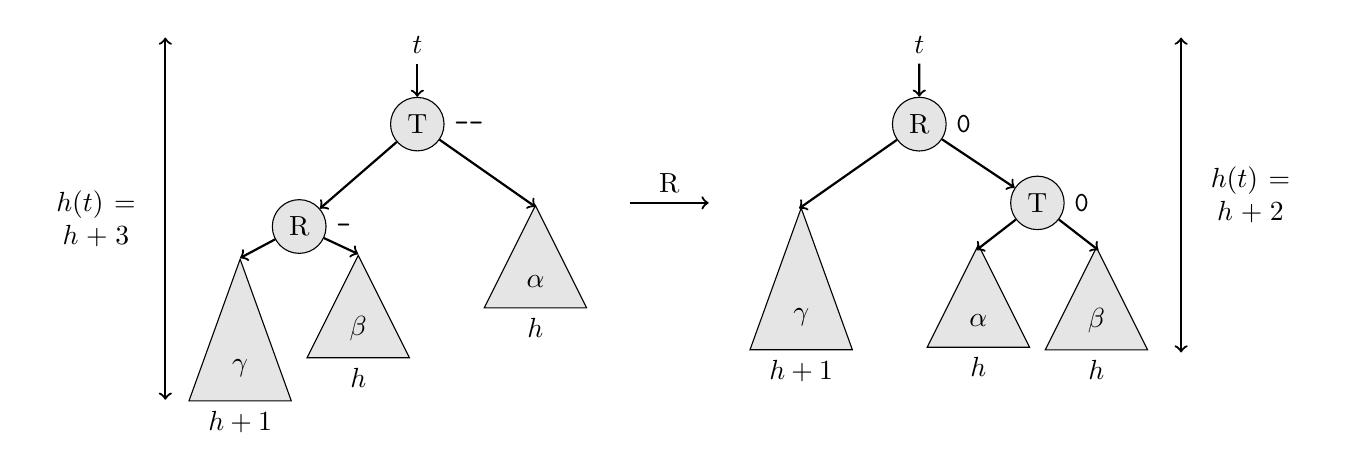
\begin{tikzpicture}[
				triangle/.style = {
					shape=isosceles triangle,
					shape border rotate = 90
				},
				level 1/.style={level distance=1cm},
				level 2/.style={sibling distance=3cm},
				level 3/.style={sibling distance=1.5cm},
				edge from parent/.style={draw=none}
			]
			\tikzstyle{Node} = [ %describes the basic look of the shapes
				text centered, 
				draw=black, 
				fill= gray!20
			]
			\tikzstyle{CircNode} = [
				circle,
				minimum width=6mm,
				Node
			]
			\tikzstyle{TriNode} = [
				triangle,
				minimum width=13mm, 
				minimum height=13mm,
				isosceles triangle stretches,
				Node
			]
			
			\node (t1) {$t$}
			child {
				node (T1) [CircNode]{T}
				child [level distance=13mm]{
					node (R1) [CircNode]{R}
					child [level distance = 18mm] {
						node (c1) [TriNode, minimum height=18mm]{$\gamma$}
					}
					child {
						node (b1) [TriNode]{$\beta$}
					}
				}
				child [level distance=20mm]{
					node (a1) [TriNode]{$\alpha$}
				}
			};
			\draw[->, thick] (t1) -- (T1);
			\draw[->, thick] (T1) -- (R1);
			\draw[->, thick] (T1) -- (1.5,-2.05);
			\draw[->, thick] (R1) -- (-0.75,-2.65);
			\draw[->, thick] (R1) -- (-2.25,-2.7);
			\node [right = 0mm of T1] {\texttt{-\hspace{0mm}-}};
			\node [right = 0mm of R1] {\texttt{-}};
			\node [below = 0mm of a1] {$h$};
			\node [below = 0mm of b1] {$h$};
			\node [below = 0mm of c1] {$h+1$};
			\draw[<->, thick] (-3.2, -4.5) -- node [anchor=center, left, text width= 1.5cm, text centered]{$h(t)=$\\$h+3$}(-3.2, 0.1);
			
			\draw[->, thick] (2.7,-2) -- (3.7,-2) node [midway, above] {R};
			
			\node (t2)[right = 6 cm of t1] {$t$}
			child {
				node (R2) [CircNode]{R}
				child[level distance = 24.5mm] {
					node (c2) [TriNode, minimum height=18mm] {$\gamma$}
				}
				child{
					node (T2) [CircNode] {T}
					[level distance = 15mm]
					child {
						node (a2) [TriNode]{$\alpha$}
					}
					child{
						node (b2)[TriNode]{$\beta$}
					}
				}
			};
			\draw[->, thick] (t2) -- (R2);
			\draw[->, thick] (R2) -- (T2);
			\draw[->, thick] (T2) -- (7.1,-2.6);
			\draw[->, thick] (T2) -- (8.65,-2.6);
			\draw[->, thick] (R2) -- (4.85,-2.07);
			\node [right = 0mm of T2] {\texttt{0}};
			\node [right = 0mm of R2] {\texttt{0}};
			\node [below = 0mm of a2] {$h$};
			\node [below = 0mm of b2] {$h$};
			\node [below = 0mm of c2] {$h+1$};
			\draw[<->, thick] (9.7, -3.9) -- node [anchor=center, right, text width= 1.5cm, text centered]{$h(t)=$\\$h+2$}(9.7, 0.1);
		\end{tikzpicture}
		\caption{Jegyezzük meg, hogy a $h(t)$ szimbólum a $t$ fa, míg a $h$ szimbólum az $\alpha$ és $\beta$ részfák magasságát jelenti.}
	\end{figure}	


	\begin{figure}[!h]
		\centering
		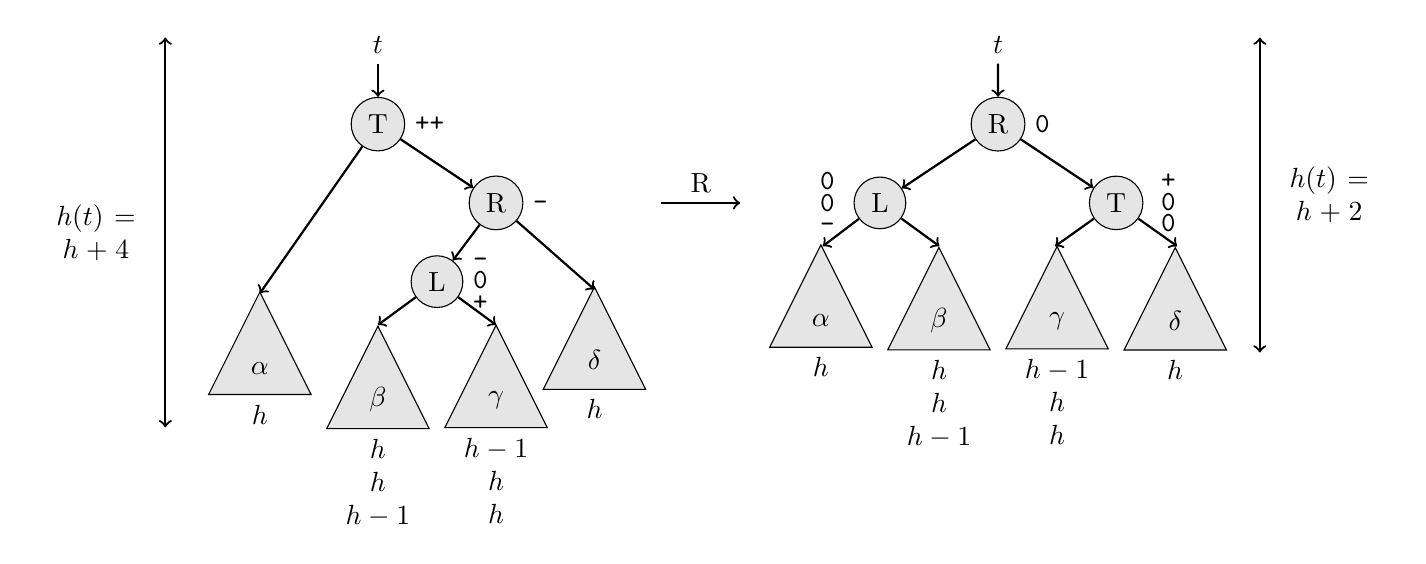
\begin{tikzpicture}[
				triangle/.style = {
					shape=isosceles triangle,
					shape border rotate = 90
				},
				level 1/.style={level distance=1cm},
				level 2/.style={sibling distance=3cm},
				level 3/.style={sibling distance=1.5cm},
				edge from parent/.style={draw=none}
			]
			\tikzstyle{Node} = [ %describes the basic look of the shapes
				text centered, 
				draw=black, 
				fill= gray!20
			]
			\tikzstyle{CircNode} = [
				circle,
				minimum width=6mm,
				Node
			]
			\tikzstyle{TriNode} = [
				triangle,
				minimum width=13mm, 
				minimum height=13mm,
				isosceles triangle stretches,
				Node
			]
			
			\node (t1) {$t$}
			child {
				node (T1) [CircNode]{T}
				child [level distance=31mm]{
					node (a1) [TriNode]{$\alpha$}
				}
				child [level distance=10mm]{
					node (R1) [CircNode]{R}
					child [level distance = 10mm] {
						node (L1) [CircNode]{L}
						child [level distance = 15mm] {
							node (b1) [TriNode]{$\beta$}
						}
						child [level distance = 15mm]{
							node (c1) [TriNode]{$\gamma$}
						}
					}
					child [level distance = 20mm, sibling distance = 25mm] {
						node (d1) [TriNode]{$\delta$}
					}
				}
			};
			\draw[->, thick] (t1) -- (T1);
			\draw[->, thick] (T1) -- (R1);
			\draw[->, thick] (R1) -- (L1);
			\draw[->, thick] (T1) -- (-1.5,-3.15);
			\draw[->, thick] (R1) -- (2.75,-3.1);
			\draw[->, thick] (L1) -- (0,-3.55);
			\draw[->, thick] (L1) -- (1.5,-3.55);
			\node [right = 0mm of T1] {\texttt{++}};
			\node [right = 0mm of R1] {\texttt{-}};
			\node [right = 0mm of L1, text width= 1.5cm] {\texttt{-}\\ \vspace{-1.5mm}\texttt{0}\\ \vspace{-1.5mm}\texttt{+}};
			\node [below = 0mm of a1] {$h$};
			\node [below = 0mm of b1, text width= 1cm, text centered] {$h$\\$h$\\$h-1$};
			\node [below = 0mm of c1, text width= 1cm, text centered] {$h-1$\\$h$\\$h$};
			\node [below = 0mm of d1] {$h$};
			\draw[<->, thick] (-2.7, -4.85) -- node [anchor=center, left, text width= 1.5cm, text centered]{$h(t)=$\\$h+4$}(-2.7, 0.1);
			
			\draw[->, thick] (3.6,-2) -- (4.6,-2) node [midway, above] {R};
			
			\node (t2) [right = 7.5cm of t1] {$t$}
			child {
				node (R2) [CircNode]{R}
				child [level distance = 10mm] {
					[level distance=15mm]
					node (L2) [CircNode]{L}
					child{
						node (a2) [TriNode]{$\alpha$}
					}
					child{
						node (b2) [TriNode]{$\beta$}
					}
				}
				child {
					[level distance=15mm]
					node (T2) [CircNode]{T}
					child {
						node (c2) [TriNode]{$\gamma$}
					}
					child{
						node (d2) [TriNode]{$\delta$}
					}
				}
			};
			\draw[->, thick] (t2) -- (R2);
			\draw[->, thick] (R2) -- (T2);
			\draw[->, thick] (R2) -- (L2);
			\draw[->, thick] (L2) -- (5.65,-2.55);
			\draw[->, thick] (L2) -- (7.13,-2.55);
			\draw[->, thick] (T2) -- (8.6,-2.55);
			\draw[->, thick] (T2) -- (10.15,-2.55);
			\node [right = 0mm of R2] {\texttt{0}};
			\node [left = 1mm of L2, text width= 2mm] {\texttt{0}\\ \vspace{-1.5mm}\texttt{0}\\ \vspace{-1.5mm}\texttt{-}};
			\node [right = 1mm of T2, text width= 1.5cm] {\texttt{+}\\ \vspace{-1.5mm}\texttt{0}\\ \vspace{-1.5mm}\texttt{0}};
			\node [below = 0mm of a2] {$h$};
			\node [below = 0mm of b2, text width= 1cm, text centered] {$h$\\$h$\\$h-1$};
			\node [below = 0mm of c2, text width= 1cm, text centered] {$h-1$\\$h$\\$h$};
			\node [below = 0mm of d2] {$h$};
			\draw[<->, thick] (11.2, -3.9) -- node [anchor=center, right, text width= 1.5cm, text centered]{$h(t)=$\\$h+2$}(11.2, 0.1);
		\end{tikzpicture}
		\caption{Jegyezzük meg, hogy a $h(t)$ szimbólum a $t$ fa, míg a $h$ szimbólum az $\alpha$ és $\beta$ részfák magasságát jelenti.}
	\end{figure}	

	\bigskip
	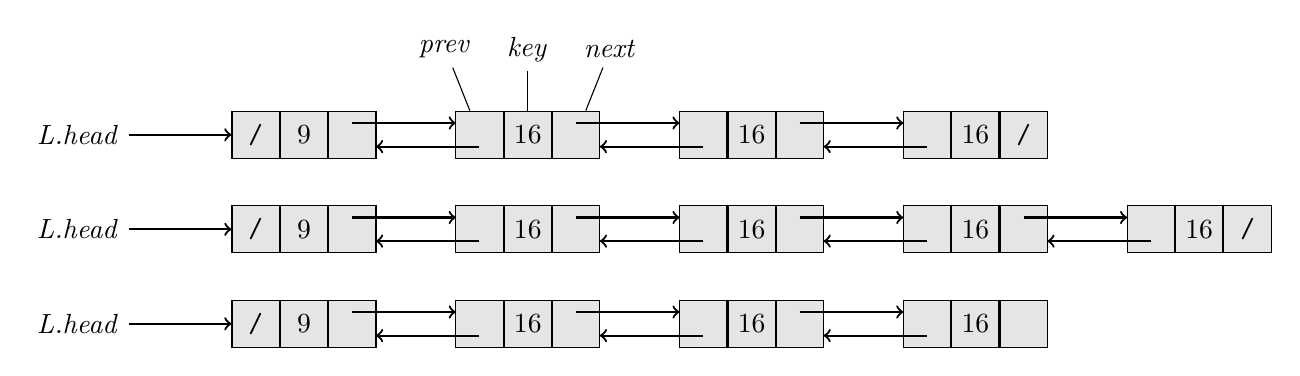
\begin{tikzpicture}
	\tikzmath{
		\x           = 0;   %dont touch this
		\y           = 0;   %dont touch this 
		\firstArrowL = 1.3; %dist between L.head and the first node
		\nodeW       = 6;   %node width
		\nodeH       = 6;   %node width
		\nodeDist    = 1;   %distance between nodes
		\figDist     = 1.2; %distance between each 
	}
	\tikzstyle{Node} = [
		minimum width=\nodeW mm, 
		minimum height=\nodeH mm, 
		text centered, 
		draw=black, 
		fill= gray!20
	]
	\tikzstyle{CircNode} =   [rectangle, Node]
	\tikzstyle{EmptyNode} = [rectangle]
	\tikzstyle{TriNode} =   [triangle, Node]
	
	\coordinate (upperArrowStart) at (0            ,+0.15);
	\coordinate (upperArrowEnd)   at (-\nodeH/2/10 ,+0.15);
	\coordinate (lowerArrowStart) at (0            ,-0.15);
	\coordinate (lowerArrowEnd)   at (+\nodeH/2/10 ,-0.15);
	
	%%%%%%%%%%%%%%%%%%%%%%%%%%===---FIRST LINE---===%%%%%%%%%%%%%%%%%%%%%%%%%%
	\node (firstHead1) [EmptyNode] at (\x,\y) {\textit{L.head}};
		\node (11l) [Node,right = \firstArrowL cm of firstHead1] {\texttt{/}};
		\node (11m) [Node,right = 0mm of 11l]                    {9};
		\node (11r) [Node,right = 0mm of 11m]                    {};
	\draw[->, thick] (firstHead1) -- (11l);
		
		\node (12l) [Node,right = \nodeDist cm of 11r]           {};
		\node (12m) [Node,right = 0mm of 12l]                    {16};
		\node (12r) [Node,right = 0mm of 12m]                    {};
	\draw[->, thick] ($(11r) + (upperArrowStart)$) -- ($(12l) + (upperArrowEnd)$);
	\draw[->, thick] ($(12l) + (lowerArrowStart)$) -- ($(11r) + (lowerArrowEnd)$);
	\node (key)  [EmptyNode, above = 5mm of 12m]                 {\textit{key}};
	\node (prev) [EmptyNode, left = 2mm of key]                  {\textit{prev}};
	\node (next) [EmptyNode, right = 2mm of key]                 {\textit{next}};
	\draw (prev) -- (12l);
	\draw (key) -- (12m);
	\draw (next) -- (12r);
	
		\node (13l) [Node,right = \nodeDist cm of 12r]           {};
		\node (13m) [Node,right = 0mm of 13l]                    {16};
		\node (13r) [Node,right = 0mm of 13m]                    {};
	\draw[->, thick] ($(12r) + (upperArrowStart)$) -- ($(13l) + (upperArrowEnd)$);
	\draw[->, thick] ($(13l) + (lowerArrowStart)$) -- ($(12r) + (lowerArrowEnd)$);
	
		\node (14l) [Node,right = \nodeDist cm of 13r]           {};
		\node (14m) [Node,right = 0mm of 14l]                    {16};
		\node (14r) [Node,right = 0mm of 14m]                    {\texttt{/}};
	\draw[->, thick] ($(13r) + (upperArrowStart)$) -- ($(14l) + (upperArrowEnd)$);
	\draw[->, thick] ($(14l) + (lowerArrowStart)$) -- ($(13r) + (lowerArrowEnd)$);
	
	%%%%%%%%%%%%%%%%%%%%%%%%%%===---SECOND LINE---===%%%%%%%%%%%%%%%%%%%%%%%%%%
	\node (firstHead2) [EmptyNode] at (\x,\y - \figDist) {\textit{L.head}};
		\node (21l) [Node,right = \firstArrowL cm of firstHead2] {\texttt{/}};
		\node (21m) [Node,right = 0mm of 21l]                    {9};
		\node (21r) [Node,right = 0mm of 21m]                    {};
	\draw[->, thick] (firstHead2) -- (21l);
	
		\node (22l) [Node,right = \nodeDist cm of 21r]           {};
		\node (22m) [Node,right = 0mm of 22l]                    {16};
		\node (22r) [Node,right = 0mm of 22m]                    {};
	\draw[->, thick] ($(21r) + (upperArrowStart)$) -- ($(22l) + (upperArrowEnd)$);
	\draw[->, thick] ($(22l) + (lowerArrowStart)$) -- ($(21r) + (lowerArrowEnd)$);
	
		\node (23l) [Node,right = \nodeDist cm of 22r]           {};
		\node (23m) [Node,right = 0mm of 23l]                    {16};
		\node (23r) [Node,right = 0mm of 23m]                    {};
	\draw[->, thick] ($(22r) + (upperArrowStart)$) -- ($(23l) + (upperArrowEnd)$);
	\draw[->, thick] ($(23l) + (lowerArrowStart)$) -- ($(22r) + (lowerArrowEnd)$);
	
		\node (24l) [Node,right = \nodeDist cm of 23r]           {};
		\node (24m) [Node,right = 0mm of 24l]                    {16};
		\node (24r) [Node,right = 0mm of 24m]                    {};
	\draw[->, thick] ($(23r) + (upperArrowStart)$) -- ($(24l) + (upperArrowEnd)$);
	\draw[->, thick] ($(24l) + (lowerArrowStart)$) -- ($(23r) + (lowerArrowEnd)$);
	
		\node (25l) [Node,right = \nodeDist cm of 24r]           {};
		\node (25m) [Node,right = 0mm of 25l]                    {16};
		\node (25r) [Node,right = 0mm of 25m]                    {\texttt{/}};
	\draw[->, thick] ($(24r) + (upperArrowStart)$) -- ($(25l) + (upperArrowEnd)$);
	\draw[->, thick] ($(25l) + (lowerArrowStart)$) -- ($(24r) + (lowerArrowEnd)$);
	
	%%%%%%%%%%%%%%%%%%%%%%%%%%===---THIRD LINE---===%%%%%%%%%%%%%%%%%%%%%%%%%%
	\node (firstHead3) [EmptyNode] at (\x,\y - 2*\figDist) {\textit{L.head}};
		\node (31l) [Node,right = \firstArrowL cm of firstHead3] {\texttt{/}};
		\node (31m) [Node,right = 0mm of 31l]                    {9};
		\node (31r) [Node,right = 0mm of 31m]                    {};
	\draw[->, thick] (firstHead3) -- (31l);
	
		\node (32l) [Node,right = \nodeDist cm of 31r]           {};
		\node (32m) [Node,right = 0mm of 32l]                    {16};
		\node (32r) [Node,right = 0mm of 32m]                    {};
	\draw[->, thick] ($(31r) + (upperArrowStart)$) -- ($(32l) + (upperArrowEnd)$);
	\draw[->, thick] ($(32l) + (lowerArrowStart)$) -- ($(31r) + (lowerArrowEnd)$);
	
		\node (33l) [Node,right = \nodeDist cm of 32r]           {};
		\node (33m) [Node,right = 0mm of 33l]                    {16};
		\node (33r) [Node,right = 0mm of 33m]                    {};
	\draw[->, thick] ($(32r) + (upperArrowStart)$) -- ($(33l) + (upperArrowEnd)$);
	\draw[->, thick] ($(33l) + (lowerArrowStart)$) -- ($(32r) + (lowerArrowEnd)$);
	
		\node (34l) [Node,right = \nodeDist cm of 33r]           {};
		\node (34m) [Node,right = 0mm of 34l]                    {16};
		\node (34r) [Node,right = 0mm of 34m]                    {};
	\draw[->, thick] ($(33r) + (upperArrowStart)$) -- ($(34l) + (upperArrowEnd)$);
	\draw[->, thick] ($(34l) + (lowerArrowStart)$) -- ($(33r) + (lowerArrowEnd)$);
	\end{tikzpicture}
\end{document}